\todo{Comm Gateway beschreiben}

\subsubsection{Mailbox Kommunikation ARM $\leftrightarrow$ NIOS2}
Die Kommunikation über die in das \ac{FPGA} programmierte Mailbox (siehe \ref{IP-Cores}) wird über eine abstrakte Klassenimplementierung in C++ dargestellt. \todo{Name, Pfad?}
Die Klasse stellt einige \textit{Write} und \textit{Read} Funktionen zur Verfügung, die mit verschiedenen Objekten umgehen können. Durch dieses Vorgehen ist sichergestellt, das der Aufrufer als Übergabeparameter nur bestimmte Objekte (die sauber definiert sind) übergegeben werden können, die auch verarbeitet werden können. Die Kommunikation erfolgt asynchron und ist intern gepuffert. Die Klasse dient als Abstraktionsschicht in beide Richtungen. Sowohl die Empfangsrichtung als auch die Senderichtung werden über die Klasse abgebildet, sodass der Aufrufer keinerlei interne Informationen über die Hardware und die Implementierung haben muss.
Nachfolgend werden die beiden wesentlichen Operationen (\textit{Write} und \textit{Read}) dargestellt und beschrieben.

\begin{figure}
	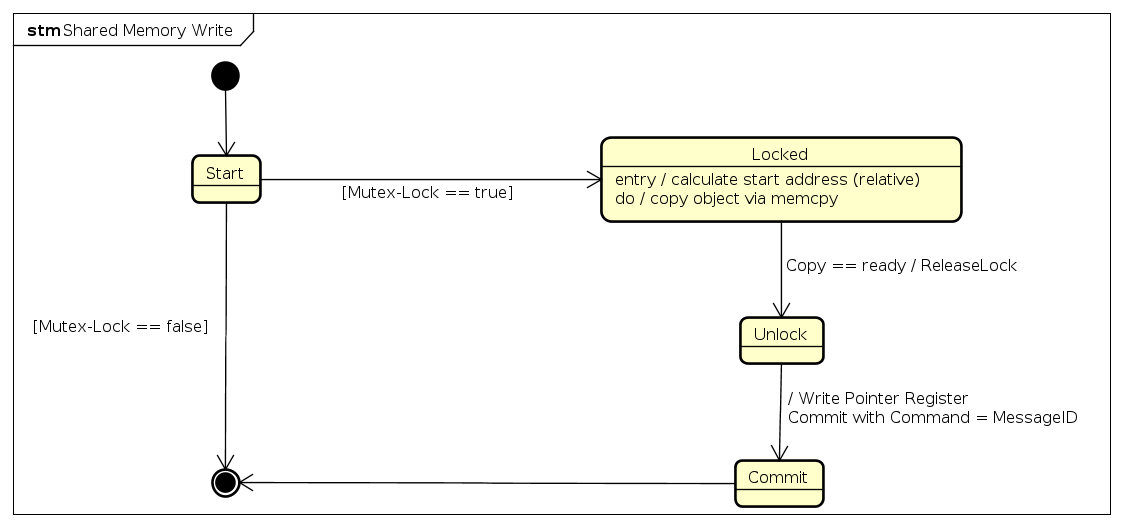
\includegraphics[width=\textwidth]{Abb/Shared_mem_Write.png}
	\caption{Schreibvorgang in den Shared Memory}
	\label{Software:Arm:SharedMemWrite}
\end{figure}

\paragraph{Write}
Der schreibende Zugriff auf den Shared Memory ist in Abbildung \ref{Software:Arm:SharedMemWrite} illustriert und hat einen einfachen Ablauf. Nachdem sich der Schreiber den Lock auf den Shared Memory über den Mutex Core geholt hat kann er Daten in diesen Bereich schreiben. Der Speicher wird dabei linear durchlaufen. Der Speicher wird dabei wie ein Ringspeicher behandelt. Ist am oberen Ende des Speichers nicht mehr genug Platz für die neue Nachricht wird wieder bei der relativen Addresse Null angefangen zu schreiben. Sind alle Daten in den Speicher geschrieben wird der Mutex wieder freigelassen. Im Speicher steht jetzt ein Abbild des Objekts, das übertragen werden soll. Es werden also nur Nutzdaten in den Speicher geschrieben. Anschließend wird die Startaddresse der Daten in das Pointer Register der Mailbox geschrieben. In das Command Register wird die eindeutige Nachrichten ID, die innerhalb des Garfield Projekts definiert ist, geschrieben. Dieser Schreibvorgang ist die letzte Instruktion zum Nachrichtenaustausch aus Sendersicht.

\paragraph{Read}
Der lesende Zugriff auf den Shared Memory ist komplizierter und unterteilt sich in zwei Abschnitte.\\

Der erste Teil der lesenden Kommunikation besteht aus dem \textbf{Interrupt}. Von dem Mailbox \ac{IP}-Core wird bei einem schreibenden Zugriff auf das Command Register automatisch ein Interrupt erzeugt. Innerhalb des \textit{ReadInterruptHandler} wird nicht der Shared Memory ausgelesen, sondern nur die Nachricht aus der Mailbox gespeichert. Die Klasse hält zusätzlich zu jedem Objekt, das verschickt bzw. empfangen werden soll einen kleinen Ringpuffer. Dieser dient dazu, die Addressen der Objekte im Shared Memory zu puffern. Tritt nun das Interrupt auf, wird zuerst das Pointer Register zwischengespeichert. Anschließend wird das Command Register, in dem der Nachrichtentyp übertragen wird, ausgelesen und anhand des Nachrichtentyps die Addresse des Pointer Registers in den passenden Puffer geschrieben. Dieses Vorgehen sorgt dafür, dass diese Funktion, die in einem Interrupthandler ausgeführt wird, sehr schnell wieder beendet ist.\\

Der zweite Teil besteht aus einem \textbf{Hintergrundtask} der zyklisch durchlaufen wird. Innerhalb dieses Task werden die Werte eines Objekts, die ausgelesen werden sollen, über eine \textit{Read} Funktion bei Bedarf überschrieben. Bei Bedarf deswegen, weil die Werte nur überschrieben werden, wenn aktuellere Werte im Shared Memory stehen. Sind aktuelle Werte verfügbar, ist der Klasseninterne Ringpuffer, der die Addressen für die Nutzdaten enthält, nicht leer. Es wird über die Addresse aus dem Shared Memory gelesen und anschließend diese Nachricht (also die Addresse) aus dem Ringpuffer entfernt.

\subsubsection{\ac{HPS} Startvorgang und Software}
Der folgende Abschnitt beschreibt die Bestandteile die für den Betrieb des ARM Dualcore notwendig sind und wie diese konfiguriert und kompiliert werden.\\

\begin{figure}
	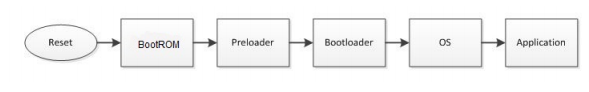
\includegraphics[width=\textwidth]{Abb/Booting.png}
	\caption{Typsicher Bootvorgang des ARM A9 Dualcore Prozessors \cite{arm_booting}}
	\label{Software:ArmBooting}
\end{figure}

Eine sehr gute und übersichtliche Beschreibung des Bootvorgangs der A9 Kerne ist in \cite{arm_booting} beschrieben. Der im \Projectname Projekt verwendeter Bootvorgang ist in Abbildung \ref{Software:ArmBooting} dargestellt. Die ersten beiden Schritte (BootRom, Preloader) sollen hier nicht weiter beschrieben werden da keine manuelle Anpassung daran notwendig ist. Als Referenz für den Buildvorgang des gesamten Systems diente \href{https://eewiki.net/display/linuxonarm/DE0-Nano-SoC+Kit}{https://eewiki.net/display/linuxonarm/DE0-Nano-SoC+Kit}. Eine komplette Kopie des Tutorials befindet sich auch im Projektverzeichnis unter \todo{Pfad}. Wenn Änderungen an der im Tutorial beschriebenden Vorgehensweise notwendig sind werden diese erwähnt.

\paragraph{Als Bootloader} kommt der beliebte U-Boot \footnote{\href{https://www.denx.de/wiki/U-Boot}{https://www.denx.de/wiki/U-Boot}} in einer leicht angepassten Variante zum Einsatz. Wie im Tutorial beschrieben werden einige Startvariablen(unter anderem das zu ladende Linux Device Tree Binary) hinzugefügt um von der SD Karte zu booten. U-Boot lädt nach dem Start dann automatisch zunächst den

\paragraph{Linux Device Tree} Der Linux Device Tree ist ein Bestandteil des Linux Kernels um eine Abstraktionsschicht zwischen Hardware (Pinouts, Speicher, Interrupts) und dem Linux Kernel zu schaffen. Durch Einsatz des Device Tree kann ein gleiches Kernel Binary auf verschiedenen Hardwareversionen und sogar komplett verschiedenen Boards benutzt werden. Der Device Tree ist eine textuelle Beschreibung der Hardware die kompiliert wird und dem Kernel beim Startvorgang übergeben wird. Ein Auszug aus einem solchen Device Tree zeigt der Code \ref{Software:DeviceTree}. Die Spezifikation des Device Trees kann man unter \href{http://www.devicetree.org/specifications/}{http://www.devicetree.org/specifications/} einsehen.

\begin{lstlisting}[caption={[Auszug aus socfpga.dtsi]Auszug aus socfpga.dtsi \cite[Version~4.7, \texttt{arch/arm/boot/dts/socfpga.dtsi}]{Linux_Kernel}}, label=Software:DeviceTree]
cpus {
	#address-cells = <1>;
	#size-cells = <0>;
	enable-method = "altr,socfpga-smp";
	
	cpu@0 {
		compatible = "arm,cortex-a9";
		device_type = "cpu";
		reg = <0>;
		next-level-cache = <&L2>;
	};
	cpu@1 {
		compatible = "arm,cortex-a9";
		device_type = "cpu";
		reg = <1>;
		next-level-cache = <&L2>;
	};
};
\end{lstlisting}

\begin{lstlisting}[caption={[Änderungen am Device Tree]Notwendige Änderungen am Device Tree}, label=Software:DevTreeGarfield]
&fpga_bridge0 {
bridge-enable = <1>;
};

&fpga_bridge1 {
bridge-enable = <1>;
};

&fpga_bridge2 {
bridge-enable = <1>;
};

/* we are extending the soc device with a specific interrupt! */
/{
soc {
mbox_rx: mailbox@0x00070000 {
compatible = "altr,mailbox-1.0";
reg = <0x70000 0x8>;
interrupt-parent = < &intc >;
interrupts = <GIC_SPI 60 4>;
#mbox-cells = <1>;
};
};

};

\end{lstlisting}
Die Änderungen, die für den Device Tree im \Projectname Projekt nötig sind, sind im Codeausschnitt \ref{Software:DevTreeGarfield} gezeigt. Es existiert außerdem eine patch-Datei, mit der der geänderte Device Tree direkt in die heruntergeladenen Kernelsourcen gepatcht und kompiliert werden kann. Die vorgenommen Änderungen ergeben sich wie folgt
\begin{itemize}
	\item fpga\_brigdes - Durch die hinzugefügten Einträge \texttt{fpga\_bridgeX} werden die verschieden verfügbaren (Achtung: Ist nur für Kernel Version 4.7 so gültig, ältere Kernel haben u.U. weniger verfügbare Bridges) Bridges beim Laden des Device Tree aktiviert.
	\item mbox\_rx - Mit diesem Eintrag wird das Interrupt, ausgelöst durch den Mailbox \ac{IP}-Core (siehe \ref{IP-Cores}) als verfügbare Hardwareeinheit dem Kernel bekanntgemacht. Interessante Attribute sind
	\begin{itemize}
		\item \texttt{@} - Die Zahl nach dem @ entspricht der Physikalischen Addresse der Mailbox. Da die Adresse im weiteren Verlauf nicht verwendet wird ist der exakte Wert nicht von Bedeutung.
		\item \texttt{compatible} - Mit diesem Attribut wird dem Interrupt ein Name gegeben. Wäre im Kernel ein generischer Hardwaretreiber für diese Mailbox vorhanden könnte dieser zur Verarbeitung genutzt werden. Wichtig für das Projekt ist der Name trotzdem, da damit das Zuordnen der Interrupt-Service-Routine zu dem Interrupt geschieht.
		\item \texttt{interrupt-parent} - Damit wird der Interrupt Controller (in unserem Fall der ARM GIC, der in einer inkludierten Beschreibungsdatei beschrieben wird) identfiziert, der das Interrupt aufnimmt und die weitere Abarbeitung in die Wege leitet.
		\item \texttt{interrupts} - Damit wird das Interrupt, das am GIC ausgelöst wird (Nummer 60) bekannt gemacht. Die Nummer ergibt sich aus: 
		\begin{itemize}
			\item Das 60te Interrupt der \textit{Shared Peripheral Interrupt} am GIC entspricht der 92ten Interruptleitung am GIC.
			\item Die 92ten Interruptleitung entspricht der 20ten Interruptleitung, die vom \ac{FPGA} verfügbar ist.
		\end{itemize} 
		\cite{interrupts_linux}.
	\end{itemize}
\end{itemize}
Die Änderungen werden direkt in die Datei arch/arm/boot/dts/socfpga\_cyclone5\_de0\_sockit.dts geschrieben.

\paragraph{Linux} wird als Betriebssystem von U-Boot geladen. Im Projekt kommt eine leicht angepasste Version der im Tutorial beschriebenen Linux Version vor. Die Änderungen sind marginal und betreffen:
\begin{itemize}
	\item Das USB-Subsystem - Zum Betrieb des \ac{Lidar} ist es notwendig einige Punkte des USB Subsystem während des Linux Kompiliervorgang (\lstinline|make menuconfig|) auszuwählen und zu kompilieren. Im groben handelt es sich um die USB-OTG Unterstützung, das ACM Subsystem und noch einige kleinere Änderungen. Auch für diesen Schritt existiert eine patch Datei im Verzeichnis \todo{Pfad}.
	\item Das \texttt{uio} Modul - Mit diesem Modul ist es möglich mit Interrupts im User-Space von Linux zu arbeiten. Dazu wird das Modul mit dem Namen, der im Device Tree angegeben wurde \lstinline|altr,mailbox-1.0| geladen. Dieses Modul erzeugt anschließend ein Gerät unter \texttt{/dev}, dass dann im User-Space genutzt werden kann. Auch diese Änderung ist in der patch Datei mit angegeben.
\end{itemize}
Als Distribution kommt eine minimale Version von Ubuntu zum Einsatz (Alternativ kann auch Debian verwendet werden). Diese Distribution wurde gewählt um einen kleine Footprint (im Leerlauf insgesammt nur ca. 35MB Arbeitsspeicherverbrauch) mit dem Komfort einer \textquotedblleft normalen\textquotedblright Linux Distribution inklusiver einem Softwarerepository zur einfachen Installation von Software zu verbinden. Sobald Linux gestartet ist kann die (hier) entscheidene Applikation

\paragraph{Comm-Gateway} gestartet werden.
\todo[inline]{Beschreibung vom Comm Gateway}
\todo{auch über interrupts im kernelspace schreiben}

\subsubsection{Empfohlener Buildvorgang und Abweichungen zum Tutorial}
Der schnellste und unkomplizierteste Weg zu einem funktionierenden Linux Image auf SD-Karte ist folgender
\begin{enumerate}
	\item Das Tutorial unter \href{https://eewiki.net/display/linuxonarm/DE0-Nano-SoC+Kit}{https://eewiki.net/display/linuxonarm/DE0-Nano-SoC+Kit} mit einer beliebigen (Mindestgröße 4GB) SD Karte durchführen. Als Kernelversion sollte unbedingt die Version 4.7 gewählt werden, da sich die im Projektrepository befindlichen Dateien darauf beziehen. Nach diesem Schritt kann man den Bootvorgang von U-Boot und Linux testen und versuchen sich im Ubuntu einzuloggen. Anschließend werden die Änderungen durchgeführt.
	\item Den Linux Devcie Tree Patchen. Dazu in einem Linux-Terminal
\lstset{language=bash}
	\begin{lstlisting}[breaklines=true]
patch socfpga-kernel-dev/KERNEL/arch/arm/boot/dts/socfpga_cyclone5_de0_sockit.dts socfpga_cyclone5_de0_sockit_garfield.patch #dieses Verzeichnis ist nach dem Tutorial verfuegbar
	\end{lstlisting}
	\item Das Linux Konfigurationsfile patchen
	\begin{lstlisting}[breaklines=true]
patch socfpga-kernel-dev/KERNEL/.config Garfield_Kernel.patch)
	\end{lstlisting}
	\item Anschließend über das Skript \texttt{socfpga-kernel-dev/tools/rebuild.sh} (oder manuell über den entsprechenden make-Befehl) den Kernel inkl. Device Tree neu kompilieren
	\item Den Linux Kernel und die Device Trees wie im Tutorial (die Punkte \texttt{Copy Kernel Image} und \texttt{Copy Kernel Device Tree Binaries}) auf die SD Karte kopieren.
\end{enumerate}

Anschließend kann man die SD-Karte wieder entnehmen und das \ac{FPGA} wieder einschalten. Das System sollte wie gewohnt starten. Um zu überprüfen, ob die Operationen funktioniert haben sollten folgenden Befehle die gleiche Ausgabe wie in Listing \todo{Verweis} haben. 
\todo{Listing einfügen, module uio und enable bridge enable}

\subsubsection{\ac{FPGA} Programmierung}
Die Programmierung des \ac{FPGA} Subsystems erfolgt unmittelbar während des Systemstarts und ist aktuell vom Softwarestart abgekoppelt. Das Image für das \ac{FPGA} wird dabei aus dem auf dem Board integrierten Flash-Speicher geladen. Die möglichen alternativen Konfigurationen sind übersichtlich im User-Manual zu dem \texttt{DE0-Nano} Board aufgelistet. Das Manual dazu findet man auf der System CD, die unter \href{http://www.terasic.com/downloads/cd-rom/de0-nano-soc/}{Link} verfügbar ist.\\

Auf dem Flash befindet sich sowohl das Image für das \ac{FPGA} als auch das executable für den nach dem flashen im \ac{FPGA} verfügbaren NIOS2. \todo{Kopie?}
\subsubsection{Applikationsstart}
Um das Kommunikationsgateway zu starten sind nach dem Login im Linux (ssh oder serielle Konsole) noch einige Schritte zu tun.
\todo[inline]{Laden der Module, starten des Servers, anschließend Verbinden zum Kommunizieren}
